
\documentclass[runningheads]{llncs}

\usepackage{graphicx}
% Used for displaying a sample figure. If possible, figure files should
% be included in EPS format.
%

\graphicspath{{./images/}}

\usepackage{hyperref}
% If you use the hyperref package, please uncomment the following line
% to display URLs in blue roman font according to Springer's eBook style:
\renewcommand\UrlFont{\color{blue}\rmfamily}

%\usepackage{courier}
\usepackage{listings, color}
\hypersetup{
  colorlinks   = true,
  linkcolor  = blue,
  citecolor  = blue,
  urlcolor   = blue
}

% nicer bold
\renewcommand{\bfdefault}{b}%

% make paragraph headings bold instead of italics
\renewcommand{\paragraph}{\textbf}%

\definecolor{dkgreen}{rgb}{0,0.6,0}
\definecolor{gray}{rgb}{0.5,0.5,0.5}
\definecolor{mauve}{rgb}{0.58,0,0.82}

\lstdefinestyle{scala}{
  language=scala,
%  basicstyle=\footnotesize\ttfamily,
  basicstyle=\scriptsize\ttfamily, % kai: temporary 
  breaklines=true,
  keywordstyle=\color{blue},
  commentstyle=\color{dkgreen},
  numbers=left,
  %frame=single, % Border around box
  %numbersep=-7pt,
  numberstyle=\color{gray},
  stringstyle=\color{mauve}
}

\lstdefinestyle{stainless}{
  numbers=none,
  breaklines=true,
  breakautoindent=true,
  breakindent=63pt,
  basicstyle=\footnotesize\ttfamily
}
 
\newcommand{\todo}[1]{{\par \color{red}#1}}


\begin{document}

\title{Towards Verifying the Bitcoin-S Library}

\author{Ramon Boss \and Kai Brünnler \and Anna Doukmak}

\authorrunning{R. Boss et al.}
\institute{Bern University of Applied Sciences, CH-2501 Biel, Switzerland
\email{\{ramon.boss,kai.bruennler,anna.doukmak\}@bfh.ch}}

\maketitle             

\begin{abstract}
  We try to verify properties of the bitcoin-s library, a Scala
  implementation of parts of the Bitcoin protocol. We use the
  Stainless verifier which supports programs in subset of Scala called
  the \emph{Pure Scala Fragment}. We first try to verify the property
  that regular transactions do not create new money. It turns out that
  there is too much code involved that lies outside of the supported
  fragment to make this feasible. However, in the process we uncover
  and fix a bug in bitcoin-s. We then turn to a much simpler (and less
  interesting) property: that adding zero satoshis to a given amount
  of satoshis yields the given amount of satoshis. Here as well a
  significant part of the relevant code lies outside of the supported
  fragment. However, after a series of equivalent transformations we
  arrive at code that we successfully verify.

\keywords{Bitcoin  \and Scala \and Bitcoin-S \and Stainless.}
\end{abstract}



\section{Introduction}

For software handling cryptocurrency, correctness is clearly crucial.
However, even in very well-tested software such as Bitcoin Core,
serious bugs occur. The most recent example is the bug found in
September 2018 \cite{cve201817144} which essentially allowed to
arbitrarily create new coins. Such software is thus a worthwhile
target for formal verification. In this work, we set out to verify
properties of the bitcoin-s library with the Stainless verifier.

\paragraph{The Bitcoin-S Library.} The bitcoin-s library is an
implementation of parts of the Bitcoin protocol in Scala
\cite{BitcoinS:website,BitcoinS:github}. In particular, it allows to
serialize, deserialize, sign and validate transactions. The library
uses immutable data structures and algebraic data types but is not
written with formal verification in mind. According to the website,
the library is used in production, handling significant amounts of
cryptocurrency each day \cite{BitcoinS:website}.

\paragraph{The Stainless Verifier.} Stainless is the successor of the
Leon verifier
\cite{DBLP:conf/ecoop/BlancKKS13,DBLP:conf/pldi/VoirolKK15,DBLP:conf/pldi/BlancK15}
and is developed at EPF Lausanne
\cite{Stainless:github}. It is intended to be
used by programmers without training in formal verification and thus
allows to write specifications in Scala and focusses on counterexample
finding in addition to proving correctness.

The following example from the Stainless documentation
\cite{Stainless:documentation} demonstrates this. Notice how a
precondition is specified using the function \emph{require} and a
postcondition using \emph{ensuring}.

\begin{lstlisting}[style=scala]
  def factorial(n: Int): Int = {
      require(n >= 0)
      if (n == 0) {
        1
      } else {
        n * factorial(n - 1)
      }
  } ensuring(res => res >= 0)
\end{lstlisting}

Our program happens not to satisfy the specification. An overflow in
the 32-bit Int leads to a negative result for the input 17, as
Stainless reports in Figure~\ref{fig:failed}. Changing the type from
Int to BigInt will result in a successful verification.

\begin{figure}
	\centering
		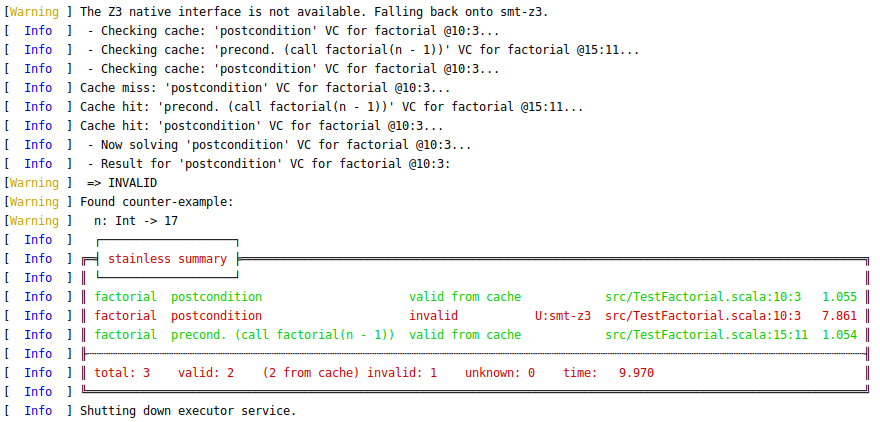
\includegraphics[width=\textwidth]{output1.png}
	\caption{Output of Stainless verification for calculating factorial of Int number}
	\label{fig:failed}
\end{figure}


\paragraph{The Pure Scala Fragment.} Stainless supports only a subset
of Scala. \todo{Anna It supports blabla, in particular it supports not
  blablabla. (check class with var)}

\todo{why does stainless use its own BigInt etc?}

They call this Pure Scala.  You can find the specification of Pure
Scala on the Stainless documentation website
\cite{Stainless:documentation} in the section
\href{https://epfl-lara.github.io/stainless/purescala.html}{Pure
  Scala}.

In addition, Stainless has its own library with annotations,
reimplementation of some core data types, collections and input-output
functions and more.  Some of them are described on the website in the
section
\href{https://epfl-lara.github.io/stainless/library.html}{Stainless
  Library}.  There are more details about the library in the source
code of Stainless on GitHub \cite{Stainless:github} in the folder
\href{https://github.com/epfl-lara/stainless/tree/master/frontends/library/stainless}{\textit{frontends/library/stainless}}.





\section{Trying to Verify the No-Inflation Property}

Thus, we try to verify the property, that a non-coinbase transaction
cannot generate new coins.  Let's name it the \nameref{property_1}.

As we can see later in chapter \ref{chap:verify_check}, we must
rewrite a huge part of the code implementing this property.  This
reimplementation into Pure Scala needs a lot of time.  So, we adjust
the plan and verify another functionality of Bitcoin-S.  Nevertheless,
during the analysis of the \nameref{property_1} we look at a bug in
Bitcoin-S found during this work and see the code changes for the
bugfix in section \ref{sec:bugfix}.


This chapter describes the part of Bitcoin-S needed to verify the
\nameref{property_1} described before.  We are going to create a
transaction and show the relevant parts of the method
\texttt{checkTransaction}, where transactions are checked against some
properties.  Then, we will see the bug in Bitcoin-S found during this
work and its fix.  In the end we see why the \nameref{property_1}
needed to be changed to the \nameref{property_2}.


\subsection{Creation of a Transaction}

Some code in this section is copied or adapted from the Bitcoin-S-Core
transaction builder example \cite{BitcoinSCore:txbuilderexample}.
Bitcoin-S-Core has a bitcoin transaction builder class with the
following constructor:
\begin{lstlisting}[style=scala, basicstyle=\scriptsize\tt]
  BitcoinTxBuilder(
    destinations: Seq[TransactionOutput], // where to send the money
    utxos: BitcoinTxBuilder.UTXOMap,      // unspent transaction outputs
    feeRate: FeeUnit,                     // fee rate per byte
    changeSPK: ScriptPubKey,              // where to send the change
    network: BitcoinNetwork               // bitcoin network information
  ): Future[BitcoinTxBuilder]
\end{lstlisting}

The return type Future does not make sense here, since the
implementation calls either Future.successful or Future.fromTry which
returns an already resolved Future.  This might be for future
purposes.

Now we create a transaction.

First, we need some money.  Thus, we create a fake transaction with
one single output.  This transaction can be parsed from the bitcoin
network, but we create one manually in order to see this process.
\begin{lstlisting}[style=scala]
  val privKey = ECPrivateKey.freshPrivateKey
  val creditingSPK = P2PKHScriptPubKey(pubKey = privKey.publicKey)

  val amount = Satoshis(Int64(10000))

  val utxo = TransactionOutput(currencyUnit = amount, scriptPubKey = creditingSPK)

  val prevTx = BaseTransaction(
    version = Int32.one,
    inputs = List.empty,
    outputs = List(utxo),
    lockTime = UInt32.zero
  )
\end{lstlisting}

On line one and two we create a new keypair to sign the next
transaction and have a scriptPubKey where the bitcoins are.  This is
our keypair.  So the money is transferred to our public key.  Line
four specifies the amount of satoshis we have in the transaction.
Then we create the actual transaction from line 6 to 13.

Now that we have some bitcoins, we create the new transaction where we
want to spend them.

First, we need some out points.  They point to outputs of previous
transactions.  We use the index zero, because the previous transaction
has only one output that becomes the first index zero.  If there were
two previous outputs, the second output would become the index 1 and
so on.
\begin{lstlisting}[style=scala]
  val outPoint = TransactionOutPoint(prevTx.txId, UInt32.zero)

  val utxoSpendingInfo = BitcoinUTXOSpendingInfo(
    outPoint = outPoint,
    output = utxo,
    signers = List(privKey),
    redeemScriptOpt = None,
    scriptWitnessOpt = None,
    hashType = HashType.sigHashAll
  )

  val utxos = List(utxoSpendingInfo)
\end{lstlisting}

This utxos are the inputs of our transaction.

Second, we need destinations to spend the bitcoins to.
For the sake of convenience we create only one.
\begin{lstlisting}[style=scala]
  val destinationAmount = Satoshis(Int64(5000))

  val destinationSPK = P2PKHScriptPubKey(pubKey = ECPrivateKey.freshPrivateKey.publicKey)

  val destinations = List(
    TransactionOutput(currencyUnit = destinationAmount, scriptPubKey = destinationSPK)
  )
\end{lstlisting}

We spend 5000 satoshis to the newly created random public key.

Finally, we define the fee rate in satoshis per one byte transaction
size as well as some bitcoin network parameters.  The bitcoin network
parameters are not important, so we use some static values normally
used when testing.

\begin{lstlisting}[style=scala]
  val feeRate = SatoshisPerByte(Satoshis.one)

  val networkParams = RegTest // some static values for testing
\end{lstlisting}

Now lets build the transaction with those data.
\begin{lstlisting}[style=scala]
  val txBuilderF: Future[BitcoinTxBuilder] = BitcoinTxBuilder(
    destinations = destinations, // where to send the money
    utxos = utxos,               // unspent transaction outputs
    feeRate = feeRate,           // fee rate per byte
    changeSPK = creditingSPK,    // where to send the change
    network = networkParams      // bitcoin network information
  )

  val signedTxF: Future[Transaction] = txBuilderF
    .flatMap(_.sign)                       // call sign on the transaction builder
    .map {
      (tx: Transaction) => println(tx.hex) // transaction in hex for the bitcoin network
    }
\end{lstlisting}

\todo{ramon: change code to get an actual transaction, completely understand and explain the code}

Line one to seven creates a transaction builder which is then signed
on line ten.  We can now use our transaction object on line twelve.
For example, after calling \emph{hex} on it, we can send the returned
string to the bitcoin network.


\subsection{Validation of a Transaction}

Bitcoin-S offers a function called \emph{checkTransaction} located in the ScriptInterpreter object.
This is its type signature:
\begin{lstlisting}[style=scala]
  checkTransaction(transaction: Transaction): Boolean
\end{lstlisting}

\begin{lstlisting}[style=scala]
/**
  * Checks the validity of a transaction in accordance to bitcoin core's CheckTransaction function
  * https://github.com/bitcoin/bitcoin/blob/f7a21dae5dbf71d5bc00485215e84e6f2b309d0a/src/main.cpp#L939.
  */
def checkTransaction(transaction: Transaction): Boolean = {
  val inputOutputsNotZero =
    !(transaction.inputs.isEmpty || transaction.outputs.isEmpty)
  val txNotLargerThanBlock = transaction.bytes.size < Consensus.maxBlockSize
  val outputsSpendValidAmountsOfMoney = !transaction.outputs.exists(o =>
    o.value < CurrencyUnits.zero || o.value > Consensus.maxMoney)

  val outputValues = transaction.outputs.map(_.value)
  val totalSpentByOutputs: CurrencyUnit =
    outputValues.fold(CurrencyUnits.zero)(_ + _)
  val allOutputsValidMoneyRange = validMoneyRange(totalSpentByOutputs)
  val prevOutputs = transaction.inputs.map(_.previousOutput)
  val noDuplicateInputs = prevOutputs.distinct.size == prevOutputs.size

  val isValidScriptSigForCoinbaseTx = transaction.isCoinbase match {
    case true =>
      transaction.inputs.head.scriptSignature.asmBytes.size >= 2 &&
        transaction.inputs.head.scriptSignature.asmBytes.size <= 100
    case false =>
      //since this is not a coinbase tx we cannot have any empty previous outs inside of inputs
      !transaction.inputs.exists(_.previousOutput == EmptyTransactionOutPoint)
  }
  inputOutputsNotZero && txNotLargerThanBlock && outputsSpendValidAmountsOfMoney && noDuplicateInputs &&
  allOutputsValidMoneyRange && noDuplicateInputs && isValidScriptSigForCoinbaseTx
}
\end{lstlisting}

We can pass a transaction and it returns a Boolean indicating whether
the transaction is valid or not.  So for example when we pass the
transaction we built before the returned value would be true, because
it's a valid transaction.  It might not be accepted by the bitcoin
network but for a transaction on its own it's valid.  We can not check
context with it, because we can only pass one transaction.

There are several checks in checkTransaction.
For example, it checks if there is either no input or no output.
In this case we get false.

The relevant part for the bug we found:
\begin{lstlisting}[style=scala]
  val prevOutputTxIds = transaction.inputs.map(_.previousOutput.txId)
  val noDuplicateInputs = prevOutputTxIds.distinct.size == prevOutputTxIds.size
\end{lstlisting}

It gathers all transaction ids referenced by the out points.  When we
call \emph{distinct} on the returned list, we get a list with
duplicate removed.  If the size of the new list is the same as the
size of the old, we know that there was no duplicate transaction id,
because, as said, distinct removes the duplicates.


\subsection{Fixing a Bug in Bitcoin-S}
\label{sec:bugfix}

We can see that there is a bug in the checkTransaction function from
before, recognized and fixed through this work.

Here is the relevant code of checkTransaction again:
\begin{lstlisting}[style=scala]
  val prevOutputTxIds = transaction.inputs.map(_.previousOutput.txId)
  val noDuplicateInputs = prevOutputTxIds.distinct.size == prevOutputTxIds.size
\end{lstlisting}

What happens if we have two TransactionOutPoints (previousOutputs) with a different index but referencing the same Transaction ID (txId)?

According to the Bitcoin protocol this is possible.  A transaction can
have multiple outputs that should be referenceable by the next
transaction.  So this is clearly a bug.

What should not be possible is a transaction referencing the same
output twice.  This bug occurred in Bitcoin Core known as
CVE-2018–17144 which was patched on September 18,
2018. \cite{cve201817144}

Here, Bitcoin-S did a bit too much and marked all transaction as
invalid, if they referenced the same transaction twice.  The fix is,
to check on TransactionOutPoint instead of TransactionOutPoint.txId,
because TransactionOutPoint contains the txId as well as the output
index it references.  So in pseudo code, we check on the tuple (tx,
index) instead of (tx).  The fixed code:
\begin{lstlisting}[style=scala]
  val prevOutputs = transaction.inputs.map(_.previousOutput)
  val noDuplicateInputs = prevOutputs.distinct.size == prevOutputs.size
\end{lstlisting}

Since TransactionOutPoint is a case class and Scala has a built in ==
for case classes there is no need to implement TransactionOutPoint.==.

This was fixed in
\href{https://github.com/bitcoin-s/bitcoin-s/pull/435}{pull request
  number 435} on GitHub at April 23, 2019, through this work along
with a unit test to prevent this bug from appearing again in the
future.


\subsection{Adjusting No-Inflation Property}

\todo{anna: what does it mean to integrate}

Trying to integrate Stainless in Bitcoin-S caused a lot of troubles,
mainly because of version conflicts.  For more details see chapter
\ref{chap:appendix_arb}.

After integrating Stainless in Bitcoin-S, there were many errors.  It
takes too much time to fix them all so it should be easier to extract
the classes needed for the \texttt{checkTransaction} function.
\todo{anna: which errors?}

The extracted code has more than 1500 lines.  After running Stainless
on it, it still throws a huge bunch of errors about what Stainless can
not reason about.  After fixing some of those errors, there appear new
ones.  So this would require changing nearly everything of the
extracted code.

Let's adjust the property from the \nameref{property_1} to the
\nameref{property_2}, because there is not enough time to fix all
these errors and write the verification.  This is way less interesting
to verify but gives still many insights in what needs to be done to
verify some parts of Bitcoin-S and other source code.

So let's look at the \nameref{property_2}.



\section{Towards Verifying the Addition-with-Zero Property}

\label{chap:verify_add}

In Bitcoin-S there is a class \texttt{Satoshis} representing an amount of bitcoins.
We look at the verification of the addition of Satoshis with zero Satoshis.
This operation should result in the same amount of Satoshis.
Let's call it the \nameref{property_2}.

Using Stainless, we see the successful verification of this property.
But the process of the verification with the tool requires many
changes in the code, so that Stainless can accept it.  We look at all
needed modifications in chapter \ref{chap:verify_add}.



After realizing that it would consume too much time to rewrite the
Bitcoin-S code and even the extracted part with checkTransaction, the
smallest unit in Bitcoin-S-Core that is worthwhile to verify was
extracted.  This could be the addition of two CurrencyUnits.  To make
it even easier, the addition of CurrencyUnits with zero.
CurrencyUnits is an abstract class in Bitcoin-S, representing
currencies like Satoshis.

\subsection{Extracting the relevant Code}

\todo{
kai text

extracted 2 files (they are in code/addition/src/main/scala/addition/original)

changes from original to reduced (new folder):
  - package name

  - removed numbers other than Int64

  - removed extending Factory, NetworkElement and BasicArithmetic. This includes some hex/byte conversion eg fromHex, hex, bytes, fromBytes, ... Just interfaces never referenced
    \href{https://bitcoin-s.org/docs/core/core-intro\#the-basics}{description in section \#the-basics (cannot add link with hashtag)}
    \href{https://github.com/bitcoin-s/bitcoin-s/blob/master/core/src/main/scala/org/bitcoins/core/protocol/NetworkElement.scala}{NetworkElement class}
    \href{https://github.com/bitcoin-s/bitcoin-s/blob/master/core/src/main/scala/org/bitcoins/core/util/Factory.scala}{Factory class}

  - removed Bitcoins class

  - removed subtraction and multiplication, binary operations <<, >>, etc, comparision operator <=, >=, etc but not == and !=

  - removed toBigDecimal

  - removed object CurrencyUnits containing some variables to transform satoshis to btc (not used)

  The code we use for the following sections is in reduced folder.
}

\todo{ramon: write this section}
\todo{ramon: keep close to original code}
\todo{ramon: for every transformation: before and after}
\todo{ramon,anna: for every transformation: why does it preserve the semantics}
\todo{ramon,anna: add comments}
\todo{ramon,anna: explain what the code does and why}

Here we can see the extracted code needed for the addition of CurrencyUnits:
\lstinputlisting[style=scala]{../code/addition/src/main/scala/addition/reduced/number/NumberType.scala}
\lstinputlisting[style=scala]{../code/addition/src/main/scala/addition/reduced/currency/CurrencyUnits.scala}

The additions' signature looks like this:
\begin{lstlisting}[style=scala]
  +(c: CurrencyUnit): CurrencyUnit
\end{lstlisting}

When we run Stainless on this code (without any properties to prove), it throws the following errors:

\begin{lstlisting}[style=stainless]
  [ Error  ] currency/CurrencyUnits.scala:6:3: Stainless doesn't support abstract type members
             type A
             ^^^^^^
  [ Error  ] currency/CurrencyUnits.scala:26:33: Only literal arguments are allowed for BigInt.
              def toBigInt: BigInt = BigInt(toLong)
                                            ^^^^^^
  [ Error  ] currency/CurrencyUnits.scala:33:1: Objects cannot extend classes or implement traits, use a case object instead
            object Satoshis extends BaseNumbers[Satoshis] {
            ^^^^^^^^^^^^^^^^^^^^^^^^^^^^^^^^^^^^^^^^^^^^^^^...
  [ Error  ] number/NumberType.scala:65:1: Objects cannot extend classes or implement traits, use a case object instead
            object Int64 extends BaseNumbers[Int64] {
            ^^^^^^^^^^^^^^^^^^^^^^^^^^^^^^^^^^^^^^^^^...
  [  Info  ] Shutting down executor service.
\end{lstlisting}

So let's see how we can fix those errors.


\subsection{Turning Object into Case Object}

Stainless output:
\begin{lstlisting}[style=stainless]
  [ Error  ] currency/CurrencyUnits.scala:33:1: Objects cannot extend classes or implement traits, use a case object instead
            object Satoshis extends BaseNumbers[Satoshis] {
            ^^^^^^^^^^^^^^^^^^^^^^^^^^^^^^^^^^^^^^^^^^^^^^^...
  [ Error  ] number/NumberType.scala:65:1: Objects cannot extend classes or implement traits, use a case object instead
            object Int64 extends BaseNumbers[Int64] {
            ^^^^^^^^^^^^^^^^^^^^^^^^^^^^^^^^^^^^^^^^^...
\end{lstlisting}

Code before:
\begin{lstlisting}[style=scala]
object Int64 extends BaseNumbers[Int64] { ... }
object Satoshis extends BaseNumbers[Satoshis] { ... }
\end{lstlisting}

Code after:
\begin{lstlisting}[style=scala]
case object Int64 extends BaseNumbers[Int64] { ... }
case object Satoshis extends BaseNumbers[Satoshis] { ... }
\end{lstlisting}

Here, we can just change the objects from object to case object.
Stainless recommendation is to use objects for modules and case objects as algebraic data types.

\todo{Ramon does this change semantics?}

This is due to the internal design of Scala.
It's possible to reason about case object but not about object.
This needs a fundamental knowledge of Scala and some functional paradigms that should not be part of this thesis.
The \href{https://github.com/epfl-lara/stainless/issues/520}{issue number 520} on Stainless GitHub gives some thoughts, if you want to know more.


\subsection{Getting Rid of Abstract Type Member}

Stainless output:
\begin{lstlisting}[style=stainless]
  [ Error  ] currency/CurrencyUnits.scala:6:3: Stainless doesn't support abstract type members
             type A
             ^^^^^^
\end{lstlisting}

This should be easy to rewrite by using generics instead of an abstract type, right?
Unfortunately not.
The problem is, CurrencyUnit uses one of its implementing classes: Satoshis.

Before:
\begin{lstlisting}[style=scala]
sealed abstract class CurrencyUnit {
  type A

  def satoshis: Satoshis

  def !=(c: CurrencyUnit): Boolean = !(this == c)

  def ==(c: CurrencyUnit): Boolean = satoshis == c.satoshis

  def +(c: CurrencyUnit): CurrencyUnit = {
    Satoshis(satoshis.underlying + c.satoshis.underlying)
  }

  protected def underlying: A
}

sealed abstract class Satoshis extends CurrencyUnit {
  override type A = Int64

  override def satoshis: Satoshis = this

  def toBigInt: BigInt = BigInt(toLong)

  def toLong: Long = underlying.toLong

  def ==(satoshis: Satoshis): Boolean = underlying == satoshis.underlying
}
\end{lstlisting}

What happens, if we typify CurrencyUnit with A, meaning to make it generic with type A?

Satoshis extends CurrencyUnit with type Int64, so it would be of type CurrencyUnit[Int64].
That's too specific, because the return type of the addition is then CurrencyUnit[Int64] not CurrencyUnit[A].
Maybe the Bitcoin-S developers should reimplement this part and not use Satoshis directly.

Since there is no easy way to fix it and the code should stay as much as possible the original, we just remove the abstract type and set it to Int64.
This limits the verification a bit, but as we only want to verify the addition in satoshis, that's OK.

After:
\begin{lstlisting}[style=scala]
sealed abstract class CurrencyUnit {
  def satoshis: Satoshis

  def !=(c: CurrencyUnit): Boolean = !(this == c)

  def ==(c: CurrencyUnit): Boolean = satoshis == c.satoshis

  def +(c: CurrencyUnit): CurrencyUnit = {
    Satoshis(satoshis.underlying + c.satoshis.underlying)
  }

  protected def underlying: Int64
}

sealed abstract class Satoshis extends CurrencyUnit {
  override def satoshis: Satoshis = this

  def toBigInt: BigInt = BigInt(toLong)

  def toLong: Long = underlying.toLong

  def ==(satoshis: Satoshis): Boolean = underlying == satoshis.underlying
}
\end{lstlisting}


\subsection{Replacing the BigInt Constructor Argument With A String Literal}

Stainless output:
\begin{lstlisting}[style=stainless]
  [ Error  ] currency/CurrencyUnits.scala:26:33: Only literal arguments are allowed for BigInt.
              def toBigInt: BigInt = BigInt(toLong)
                                            ^^^^^^
\end{lstlisting}

As described before, Stainless supports only a subset of Scala.
The BigInt from the Stainless library is a bit restricted.
One such restriction is, that BigInt does not support dynamic BigInt construction.
Thus, the constructor parameter of BitInt must be a literal argument.

Before:
\begin{lstlisting}[style=scala]
sealed abstract class Satoshis extends CurrencyUnit {
  override def satoshis: Satoshis = this

  def toBigInt: BigInt = BigInt(toLong)

  def toLong: Long = underlying.toLong

  def ==(satoshis: Satoshis): Boolean = underlying == satoshis.underlying
}
\end{lstlisting}

After:
\begin{lstlisting}[style=scala]
sealed abstract class Satoshis extends CurrencyUnit {
  override def satoshis: Satoshis = this

  def toBigInt: BigInt = underlying.toBigInt

  def toLong: Long = underlying.toLong

  def ==(satoshis: Satoshis): Boolean = underlying == satoshis.underlying
}
\end{lstlisting}

This would be really hard to refactor, because Bitcoin-S tries to be as dynamic as possible so it can be used with cryptocurrencies other than bitcoins.
Maybe it could be impossible, because they need to parse dynamic values from the bitcoin network.

Luckily, we can use toBigInt on the field \texttt{underlying} directly instead of toLong.
So, instead of converting the underlying to Long and back to BigInt we convert underlying directly to BigInt.

After fixing all Stainless errors, a new error appears.


\subsection{Getting Rid of Special Generics}

Stainless output:
\begin{lstlisting}[style=stainless]
  [ Error  ] number/NumberType.scala:8:30: Unknown type parameter type T
  sealed abstract class Number[T <: Number[T]] {
                               ^^^^^^^^^^^^^^

\end{lstlisting}

This is a missing feature in Stainless.
It does not support upper type boundaries on the class itself.
To track this, \href{https://github.com/epfl-lara/stainless/issues/519}{issue 519} was created on GitHub during this work.

Before:
\begin{lstlisting}[style=scala]
sealed abstract class Number[T <: Number[T]] {
  type A = BigInt

  /** The underlying scala number used to to hold the number */
  protected def underlying: A

  def toLong: Long = toBigInt.bigInteger.longValueExact()
  def toBigInt: BigInt = underlying

  /**
    * This is used to determine the valid amount of bytes in a number
    * for instance a UInt8 has an andMask of 0xff
    * a UInt32 has an andMask of 0xffffffff
    */
  def andMask: BigInt

  /** Factory function to create the underlying T, for instance a UInt32 */
  def apply: A => T

  def +(num: T): T = apply(checkResult(underlying + num.underlying))

  /**
    * Checks if the given result is within the range
    * of this number type
    */
  private def checkResult(result: BigInt): A = {
    require((result & andMask) == result,
      "Result was out of bounds, got: " + result)
    result
  }
}

/**
  * Represents a signed number in our number system
  * Instances of this is [[Int64]]
  */
sealed abstract class SignedNumber[T <: Number[T]] extends Number[T]

/**
  * Represents a int64_t in C
  */
sealed abstract class Int64 extends SignedNumber[Int64] {
  override def apply: A => Int64 = Int64(_)
  override def andMask = 0xffffffffffffffffL
}
\end{lstlisting}

After:
\begin{lstlisting}[style=scala]
sealed abstract class Number {
  type A = BigInt

  /** The underlying scala number used to to hold the number */
  protected def underlying: A

  def toLong: Long = toBigInt.bigInteger.longValueExact()
  def toBigInt: BigInt = underlying

  /**
    * This is used to determine the valid amount of bytes in a number
    * for instance a UInt8 has an andMask of 0xff
    * a UInt32 has an andMask of 0xffffffff
    */
  def andMask: BigInt

  /** Factory function to create the underlying T, for instance a UInt32 */
  def apply: A => Int64

  def +(num: Int64): Int64 = apply(checkResult(underlying + num.underlying))

  /**
    * Checks if the given result is within the range
    * of this number type
    */
  private def checkResult(result: BigInt): A = {
    require((result & andMask) == result,
      "Result was out of bounds, got: " + result)
    result
  }
}

/**
  * Represents a signed number in our number system
  * Instances of this is [[Int64]]
  */
sealed abstract class SignedNumber extends Number

/**
  * Represents a int64_t in C
  */
sealed abstract class Int64 extends SignedNumber {
  override def apply: A => Int64 = Int64(_)
  override def andMask = 0xffffffffffffffffL
}
\end{lstlisting}

Despite this, in order to be able to continue, we make this a concrete type by replacing T with Int64.
Int64,  because Satoshis uses only Int64.
There are other number types like UInt16 but for our property we don't need them.

Now, there are two new errors.


\subsection{Removing toLong}

Stainless output:
\begin{lstlisting}[style=stainless]
  [ Error  ] number/NumberType.scala:14:22: Unknown call to bigInteger on Number.this.toBigInt (BigInt) with arguments List() of type List()
             def toLong: Long = toBigInt.bigInteger.longValueExact()
                                ^^^^^^^^^^^^^^^^^^^
\end{lstlisting}


Now that we do not depend on toLong anymore lets just remove it from out code.

Before:
\begin{lstlisting}[style=scala]
sealed abstract class Satoshis extends CurrencyUnit {
  override def satoshis: Satoshis = this

  def toBigInt: BigInt = underlying.toBigInt

  def toLong: Long = underlying.toLong

  def ==(satoshis: Satoshis): Boolean = underlying == satoshis.underlying
}  
\end{lstlisting}

After:
\begin{lstlisting}[style=scala]
sealed abstract class Satoshis extends CurrencyUnit {
  override def satoshis: Satoshis = this

  def toBigInt: BigInt = underlying.toBigInt

  def ==(satoshis: Satoshis): Boolean = underlying == satoshis.underlying
}  
\end{lstlisting}

And before:
\begin{lstlisting}[style=scala]
sealed abstract class Number {
  type A = BigInt

  /** The underlying scala number used to to hold the number */
  protected def underlying: A

  def toLong: Long = toBigInt.bigInteger.longValueExact()
  def toBigInt: BigInt = underlying

  /**
    * This is used to determine the valid amount of bytes in a number
    * for instance a UInt8 has an andMask of 0xff
    * a UInt32 has an andMask of 0xffffffff
    */
  def andMask: BigInt

  /** Factory function to create the underlying T, for instance a UInt32 */
  def apply: A => Int64

  def +(num: Int64): Int64 = apply(checkResult(underlying + num.underlying))

  /**
    * Checks if the given result is within the range
    * of this number type
    */
  private def checkResult(result: BigInt): A = {
    require((result & andMask) == result,
      "Result was out of bounds, got: " + result)
    result
  }
}  
\end{lstlisting}

After:
\begin{lstlisting}[style=scala]
sealed abstract class Number {
  type A = BigInt

  /** The underlying scala number used to to hold the number */
  protected def underlying: A

  def toBigInt: BigInt = underlying

  /**
    * This is used to determine the valid amount of bytes in a number
    * for instance a UInt8 has an andMask of 0xff
    * a UInt32 has an andMask of 0xffffffff
    */
  def andMask: BigInt

  /** Factory function to create the underlying T, for instance a UInt32 */
  def apply: A => Int64

  def +(num: Int64): Int64 = apply(checkResult(underlying + num.underlying))

  /**
    * Checks if the given result is within the range
    * of this number type
    */
  private def checkResult(result: BigInt): A = {
    require((result & andMask) == result,
      "Result was out of bounds, got: " + result)
    result
  }
}
\end{lstlisting}


\subsection{Getting Rid of Concrete Type}

Stainless output:
\begin{lstlisting}[style=stainless]
  [Warning ] number/NumberType.scala:9:3: Could not extract tree in class: type A = BigInt (class scala.reflect.internal.Trees$TypeDef)
               type A = BigInt
               ^^^^^^^^^^^^^^^

\end{lstlisting}

Before:
\begin{lstlisting}[style=scala]
sealed abstract class Number {
  type A = BigInt

  /** The underlying scala number used to to hold the number */
  protected def underlying: A

  def toBigInt: BigInt = underlying

  /** Factory function to create the underlying T, for instance a UInt32 */
  def apply: A => Int64

  def +(num: Int64): Int64 = apply(checkResult(underlying + num.underlying))

  /**
    * Checks if the given result is within the range
    * of this number type
    */
  private def checkResult(result: BigInt): A = {
    require(
          result <= BigInt("9223372036854775807")
      && result >= BigInt("-9223372036854775808"))
    result
  }
}

/**
  * Represents a signed number in our number system
  * Instances of this is [[Int64]]
  */
sealed abstract class SignedNumber extends Number

/**
  * Represents a int64_t in C
  */
sealed abstract class Int64 extends SignedNumber {
  override def apply: A => Int64 = Int64(_)
}  
\end{lstlisting}

After:
\begin{lstlisting}[style=scala]
sealed abstract class Number {
  /** The underlying scala number used to to hold the number */
  protected def underlying: BigInt

  def toBigInt: BigInt = underlying

  /** Factory function to create the underlying T, for instance a UInt32 */
  def apply: BigInt => Int64

  def +(num: Int64): Int64 = apply(checkResult(underlying + num.underlying))

  /**
    * Checks if the given result is within the range
    * of this number type
    */
  private def checkResult(result: BigInt): BigInt = {
    require(
         result <= BigInt("9223372036854775807")
      && result >= BigInt("-9223372036854775808"))
    result
  }
}

/**
  * Represents a signed number in our number system
  * Instances of this is [[Int64]]
  */
sealed abstract class SignedNumber extends Number

/**
  * Represents a int64_t in C
  */
sealed abstract class Int64 extends SignedNumber {
  override def apply: BigInt => Int64 = Int64(_)
}
\end{lstlisting}

This is easy.
We just replace all occurrence of A with BigInt, since A is not overwritten in an implementing class.
This is not the exact same code, because an implementing class can not override A anymore but that's fine for our verification.

This was a missing feature in Stainless that was fixed on Mai 28, 2019 with \href{https://github.com/epfl-lara/stainless/pull/470}{pull request 470} on GitHub.
Now it should work without this change.


\subsection{Replacing the BigInt \&-Function With Bound Check}
\label{sec:bound_check}

Stainless output:
\begin{lstlisting}[style=stainless]
  [ Error  ] number/NumberType.scala:33:14: Unknown call to & on result (BigInt) with arguments List(Number.this.andMask) of type List(BigInt)
               require((result & andMask) == result,
                       ^^^^^^^^^^^^^^^^

\end{lstlisting}

Due to the restrictions on BigInt, we can not use the \& function either.
Before:
\begin{lstlisting}[style=scala]
sealed abstract class Number {
  type A = BigInt

  /** The underlying scala number used to to hold the number */
  protected def underlying: A

  def toBigInt: BigInt = underlying

  /**
    * This is used to determine the valid amount of bytes in a number
    * for instance a UInt8 has an andMask of 0xff
    * a UInt32 has an andMask of 0xffffffff
    */
  def andMask: BigInt

  /** Factory function to create the underlying T, for instance a UInt32 */
  def apply: A => Int64

  def +(num: Int64): Int64 = apply(checkResult(underlying + num.underlying))

  /**
    * Checks if the given result is within the range
    * of this number type
    */
  private def checkResult(result: BigInt): A = {
    require((result & andMask) == result,
      "Result was out of bounds, got: " + result)
    result
  }
}

/**
  * Represents a signed number in our number system
  * Instances of this is [[Int64]]
  */
sealed abstract class SignedNumber extends Number

/**
  * Represents a int64_t in C
  */
sealed abstract class Int64 extends SignedNumber {
  override def apply: A => Int64 = Int64(_)
  override def andMask = 0xffffffffffffffffL
}
\end{lstlisting}

After:
\begin{lstlisting}[style=scala]
sealed abstract class Number {
  type A = BigInt

  /** The underlying scala number used to to hold the number */
  protected def underlying: A

  def toBigInt: BigInt = underlying

  /** Factory function to create the underlying T, for instance a UInt32 */
  def apply: A => Int64

  def +(num: Int64): Int64 = apply(checkResult(underlying + num.underlying))

  /**
    * Checks if the given result is within the range
    * of this number type
    */
  private def checkResult(result: BigInt): A = {
    require(
          result <= BigInt("9223372036854775807")
      && result >= BigInt("-9223372036854775808"),
      "Result was out of bounds, got: " + result)
    result
  }
}

/**
  * Represents a signed number in our number system
  * Instances of this is [[Int64]]
  */
sealed abstract class SignedNumber extends Number

/**
  * Represents a int64_t in C
  */
sealed abstract class Int64 extends SignedNumber {
  override def apply: A => Int64 = Int64(_)
}
\end{lstlisting}

This is a bounds check.
It checks if the result of the addition is in range of the specified type, which is now the hard coded Int64.

So, we can replace the \& mask with a bound check whether the result is in range of Long.MinValue and Long.MaxValue, because Int64 has the same 64-bit range as Long.
Again the code gets a bit more static and it's not the exact same code anymore.

Running Stainless produces again new errors.


\subsection{Extracting Private Inner Classes}

Stainless output:
\begin{lstlisting}[style=stainless]
  [Warning ] currency/CurrencyUnits.scala:36:3: Could not extract tree in class: case private class SatoshisImpl extends Satoshis with Product with Serializable {
  [Warning ]   <caseaccessor> <paramaccessor> private[this] val underlying: addition.modified.number.Int64 = _;
  [Warning ]   <stable> <caseaccessor> <accessor> <paramaccessor> def underlying: addition.modified.number.Int64 = SatoshisImpl.this.underlying;
  [Warning ]   def <init>(underlying: addition.modified.number.Int64): addition.modified.currency.Satoshis.SatoshisImpl = {
  [Warning ]     SatoshisImpl.super.<init>();
  [Warning ]     ()
  [Warning ]   };
  [Warning ]   <synthetic> def copy(underlying: addition.modified.number.Int64 = underlying): addition.modified.currency.Satoshis.SatoshisImpl = new SatoshisImpl(underlying);
  [Warning ]   <synthetic> def copy$default$1: addition.modified.number.Int64 = SatoshisImpl.this.underlying;
  [Warning ]   override <synthetic> def productPrefix: String = "SatoshisImpl";
  [Warning ]   <synthetic> def productArity: Int = 1;
  [Warning ]   <synthetic> def productElement(x$1: Int): Any = x$1 match {
  [Warning ]     case 0 => SatoshisImpl.this.underlying
  [Warning ]     case _ => throw new IndexOutOfBoundsException(x$1.toString())
  [Warning ]   };
  [Warning ]   override <synthetic> def productIterator: Iterator[Any] = runtime.this.ScalaRunTime.typedProductIterator[Any](SatoshisImpl.this);
  [Warning ]   <synthetic> def canEqual(x$1: Any): Boolean = x$1.$isInstanceOf[addition.modified.currency.Satoshis.SatoshisImpl]();
  [Warning ]   override <synthetic> def hashCode(): Int = ScalaRunTime.this._hashCode(SatoshisImpl.this);
  [Warning ]   override <synthetic> def toString(): String = ScalaRunTime.this._toString(SatoshisImpl.this);
  [Warning ]   override <synthetic> def equals(x$1: Any): Boolean = SatoshisImpl.this.eq(x$1.asInstanceOf[Object]).||(x$1 match {
  [Warning ]   case (_: addition.modified.currency.Satoshis.SatoshisImpl) => true
  [Warning ]   case _ => false
  [Warning ] }.&&({
  [Warning ]     <synthetic> val SatoshisImpl$1: addition.modified.currency.Satoshis.SatoshisImpl = x$1.asInstanceOf[addition.modified.currency.Satoshis.SatoshisImpl];
  [Warning ]     SatoshisImpl.this.underlying.==(SatoshisImpl$1.underlying).&&(SatoshisImpl$1.canEqual(SatoshisImpl.this))
  [Warning ]   }))
  [Warning ] } (class scala.reflect.internal.Trees$ClassDef)
                private case class SatoshisImpl(underlying: Int64) extends Satoshis
                ^^^^^^^^^^^^^^^^^^^^^^^^^^^^^^^^^^^^^^^^^^^^^^^^^^^^^^^^^^^^^^^^^^^
\end{lstlisting}

And:
\begin{lstlisting}[style=stainless]
  [Warning ] number/NumberType.scala:59:3: Could not extract tree in class: case private class Int64Impl extends Int64 with Product with Serializable {
    [Warning ]   <caseaccessor> <paramaccessor> private[this] val underlying: BigInt = _;
    [Warning ]   <stable> <caseaccessor> <accessor> <paramaccessor> def underlying: BigInt = Int64Impl.this.underlying;
    [Warning ]   def <init>(underlying: BigInt): addition.modified.number.Int64.Int64Impl = {
    [Warning ]     Int64Impl.super.<init>();
    [Warning ]     ()
    [Warning ]   };
    [Warning ]   scala.this.Predef.require(Int64Impl.this.underlying.>=(math.this.BigInt.long2bigInt(-9223372036854775808L)), "Number was too small for a int64, got: ".+(Int64Impl.this.underlying));
    [Warning ]   scala.this.Predef.require(Int64Impl.this.underlying.<=(math.this.BigInt.long2bigInt(9223372036854775807L)), "Number was too big for a int64, got: ".+(Int64Impl.this.underlying));
    [Warning ]   <synthetic> def copy(underlying: BigInt = underlying): addition.modified.number.Int64.Int64Impl = new Int64Impl(underlying);
    [Warning ]   <synthetic> def copy$default$1: BigInt = Int64Impl.this.underlying;
    [Warning ]   override <synthetic> def productPrefix: String = "Int64Impl";
    [Warning ]   <synthetic> def productArity: Int = 1;
    [Warning ]   <synthetic> def productElement(x$1: Int): Any = x$1 match {
    [Warning ]     case 0 => Int64Impl.this.underlying
    [Warning ]     case _ => throw new IndexOutOfBoundsException(x$1.toString())
    [Warning ]   };
    [Warning ]   override <synthetic> def productIterator: Iterator[Any] = runtime.this.ScalaRunTime.typedProductIterator[Any](Int64Impl.this);
    [Warning ]   <synthetic> def canEqual(x$1: Any): Boolean = x$1.$isInstanceOf[addition.modified.number.Int64.Int64Impl]();
    [Warning ]   override <synthetic> def hashCode(): Int = ScalaRunTime.this._hashCode(Int64Impl.this);
    [Warning ]   override <synthetic> def toString(): String = ScalaRunTime.this._toString(Int64Impl.this);
    [Warning ]   override <synthetic> def equals(x$1: Any): Boolean = Int64Impl.this.eq(x$1.asInstanceOf[Object]).||(x$1 match {
    [Warning ]   case (_: addition.modified.number.Int64.Int64Impl) => true
    [Warning ]   case _ => false
    [Warning ] }.&&({
    [Warning ]     <synthetic> val Int64Impl$1: addition.modified.number.Int64.Int64Impl = x$1.asInstanceOf[addition.modified.number.Int64.Int64Impl];
    [Warning ]     Int64Impl.this.underlying.==(Int64Impl$1.underlying).&&(Int64Impl$1.canEqual(Int64Impl.this))
    [Warning ]   }))
    [Warning ] } (class scala.reflect.internal.Trees$ClassDef)
                 private case class Int64Impl(underlying: BigInt) extends Int64 {
                 ^^^^^^^^^^^^^^^^^^^^^^^^^^^^^^^^^^^^^^^^^^^^^^^^^^^^^^^^^^^^^^^^...
\end{lstlisting}

Stainless can not extract the private class inside the object.
Bitcoin-S uses this a lot, because they separate the class from its implementation.

Before:
\begin{lstlisting}[style=scala]
case object Satoshis extends BaseNumbers[Satoshis] {
  val min = Satoshis(Int64.min)
  val max = Satoshis(Int64.max)
  val zero = Satoshis(Int64.zero)
  val one = Satoshis(Int64.one)

  def apply(int64: Int64): Satoshis = SatoshisImpl(int64)

  private case class SatoshisImpl(underlying: Int64) extends Satoshis
}
\end{lstlisting}

After:
\begin{lstlisting}[style=scala]
case object Satoshis extends BaseNumbers[Satoshis] {

  val min = Satoshis(Int64.min)
  val max = Satoshis(Int64.max)
  val zero = Satoshis(Int64.zero)
  val one = Satoshis(Int64.one)

  def apply(int64: Int64): Satoshis = SatoshisImpl(int64)
}

private case class SatoshisImpl(underlying: Int64) extends Satoshis
\end{lstlisting}

And before:
\begin{lstlisting}[style=scala]
case object Int64 extends BaseNumbers[Int64] {
  private case class Int64Impl(underlying: BigInt) extends Int64 {
    require(underlying >= -9223372036854775808L,
      "Number was too small for a int64, got: " + underlying)
    require(underlying <= 9223372036854775807L,
      "Number was too big for a int64, got: " + underlying)
  }

  lazy val zero = Int64(0)
  lazy val one = Int64(1)

  lazy val min = Int64(-9223372036854775808L)
  lazy val max = Int64(9223372036854775807L)

  def apply(long: Long): Int64 = Int64(BigInt(long))

  def apply(bigInt: BigInt): Int64 = Int64Impl(bigInt)
}
\end{lstlisting}

After:
\begin{lstlisting}[style=scala]
case object Int64 extends BaseNumbers[Int64] {
  lazy val zero = Int64(0)
  lazy val one = Int64(1)

  lazy val min = Int64(-9223372036854775808L)
  lazy val max = Int64(9223372036854775807L)

  def apply(long: Long): Int64 = Int64(BigInt(long))

  def apply(bigInt: BigInt): Int64 = Int64Impl(bigInt)
}

private case class Int64Impl(underlying: BigInt) extends Int64 {
  require(underlying >= -9223372036854775808L,
    "Number was too small for a int64, got: " + underlying)
  require(underlying <= 9223372036854775807L,
    "Number was too big for a int64, got: " + underlying)
}
\end{lstlisting}

This is easy to fix.
We just extract the private class out of the object.
This is not exactly the same code, because other classes in the same file could now access the private class.
But for our property it does not change anything.

Now we get some weird warnings about require.


\subsection{Removing Second Parameter of Require}

Stainless output:
\begin{lstlisting}[style=stainless]
  [Warning ] number/NumberType.scala:9:3: Could not extract tree in class: type A = BigInt (class scala.reflect.internal.Trees$TypeDef)
            type A = BigInt
            ^^^^^^^^^^^^^^^
  [Warning ] number/NumberType.scala:71:3: Could not extract tree in class: scala.this.Predef.require(Int64Impl.this.underlying.>=(math.this.BigInt.long2bigInt(-9223372036854775808L)), "Number was too small for a int64, got: ".+(Int64Impl.this.underlying)) (class scala.reflect.internal.Trees$Apply)
            require(underlying >= -9223372036854775808L,
            ^^^^^^^^^^^^^^^^^^^^^^^^^^^^^^^^^^^^^^^^^^^^...
  [Warning ] number/NumberType.scala:73:3: Could not extract tree in class: scala.this.Predef.require(Int64Impl.this.underlying.<=(math.this.BigInt.long2bigInt(9223372036854775807L)), "Number was too big for a int64, got: ".+(Int64Impl.this.underlying)) (class scala.reflect.internal.Trees$Apply)
            require(underlying <= 9223372036854775807L,
            ^^^^^^^^^^^^^^^^^^^^^^^^^^^^^^^^^^^^^^^^^^^...
  [ Error  ] checkResult$0 depends on missing dependencies: require$1.

\end{lstlisting}

Seems like Stainless does not support the second string parameter of require or at least it throws a warning about it.
We can safely remove the string parameters from the requires, since they only serve as error messages.

Before:
\begin{lstlisting}[style=scala]
private case class Int64Impl(underlying: BigInt) extends Int64 {
  require(underlying >= -9223372036854775808L,
    "Number was too small for a int64, got: " + underlying)
  require(underlying <= 9223372036854775807L,
    "Number was too big for a int64, got: " + underlying)
}
\end{lstlisting}

After:
\begin{lstlisting}[style=scala]
private case class Int64Impl(underlying: BigInt) extends Int64 {
  require(underlying >= -9223372036854775808L)
  require(underlying <= 9223372036854775807L)
}
\end{lstlisting}

And before:
\begin{lstlisting}[style=scala]
sealed abstract class Number {
  type A = BigInt

  /** The underlying scala number used to to hold the number */
  protected def underlying: A

  def toBigInt: BigInt = underlying

  /** Factory function to create the underlying T, for instance a UInt32 */
  def apply: A => Int64

  def +(num: Int64): Int64 = apply(checkResult(underlying + num.underlying))

  /**
    * Checks if the given result is within the range
    * of this number type
    */
  private def checkResult(result: BigInt): A = {
    require(
         result <= BigInt("9223372036854775807")
      && result >= BigInt("-9223372036854775808"),
      "Result was out of bounds, got: " + result)
    result
  }
}
\end{lstlisting}

After:
\begin{lstlisting}[style=scala]
sealed abstract class Number {
  type A = BigInt

  /** The underlying scala number used to to hold the number */
  protected def underlying: A

  def toBigInt: BigInt = underlying

  /** Factory function to create the underlying T, for instance a UInt32 */
  def apply: A => Int64

  def +(num: Int64): Int64 = apply(checkResult(underlying + num.underlying))

  /**
    * Checks if the given result is within the range
    * of this number type
    */
  private def checkResult(result: BigInt): A = {
    require(
          result <= BigInt("9223372036854775807")
      && result >= BigInt("-9223372036854775808"))
    result
  }
}
\end{lstlisting}

A new error appears.


\subsection{Rewriting BigInt to Long Conversions}

Stainless output:
\begin{lstlisting}[style=stainless]
  [ Error  ] inv$4 depends on missing dependencies: long2bigInt$0.
  [ Error  ] apply$14 depends on missing dependencies: BigInt$0, apply$15.
\end{lstlisting}

This error is hard to understand, but we can see that there is a missing Long to BigInt conversion.
So we search for all Long values in the code.

Before:
\begin{lstlisting}[style=scala]
private case class Int64Impl(underlying: BigInt) extends Int64 {
  require(underlying >= -9223372036854775808L)
  require(underlying <= 9223372036854775807L)
}
\end{lstlisting}

After:
\begin{lstlisting}[style=scala]
private case class Int64Impl(underlying: BigInt) extends Int64 {
  require(underlying >= BigInt("-9223372036854775808"))
  require(underlying <= BigInt("9223372036854775807"))
}  
\end{lstlisting}

And before:
\begin{latlisting}[style=scala]
case object Int64 extends BaseNumbers[Int64] {
  lazy val zero = Int64(0)
  lazy val one = Int64(1)

  lazy val min = Int64(-9223372036854775808L)
  lazy val max = Int64(9223372036854775807L)

  def apply(long: Long): Int64 = Int64(BigInt(long))

  def apply(bigInt: BigInt): Int64 = Int64Impl(bigInt)
}
\end{latlisting}

After:
\begin{lstlisting}[style=scala]
case object Int64 extends BaseNumbers[Int64] {
  lazy val zero = Int64(0)
  lazy val one = Int64(1)

  lazy val min = Int64(BigInt("-9223372036854775808"))
  lazy val max = Int64(BigInt("9223372036854775807"))

  def apply(bigInt: BigInt): Int64 = Int64Impl(bigInt)
}
\end{lstlisting}

Looks like it can not compare a BigInt with a Long value.
We can easily convert this Long value to a BigInt with a string literal parameter by passing these numbers as strings to the BigInt constructor.

Finally, we get some output from Stainless about the verification in the code.
\begin{lstlisting}[style=stainless]
[...]
[Warning ]  => INVALID
[Warning ] Found counter-example:
[Warning ]   thiss: { x: Object | @unchecked isNumber(x) } -> Int64Impl(0)
[Warning ]   num: { x: Object | @unchecked isInt64(x) }    -> Int64Impl(9223372036854775808)
[...]
[  Info  ] +  precond. (call checkResult(thiss, underlying(thiss) + u ...)  invalid  Code.scala:16:45
[...]
[  Info  ] total: 5  valid: 4  (4 from cache) invalid: 1  unknown: 0  time:  1.317
\end{lstlisting}

This shows that there is an invalid specification in checkResult and Stainless prints a counterexample for it.

Let's ignore this for a moment and write the specification for the \nameref{property_2}.


\subsection{Writing Specification for the Property}

As specified, our verification must only support addition with zero.
So we restrict the parameter to be zero in the precondition.
\begin{lstlisting}[style=scala]
  require(c.satoshis == Satoshis.zero)
\end{lstlisting}

We ensure the result is the same value as \emph{this} in the postcondition.
\begin{lstlisting}[style=scala]
  ensuring(res => res.satoshis == this.satoshis)
\end{lstlisting}

We can use equals (==) directly on Satoshis, because it is a case class.
The addition will now look like this:
\begin{lstlisting}[style=scala]
  override def +(c: CurrencyUnit): CurrencyUnit = {
    require(c.satoshis == Satoshis.zero)
    Satoshis(satoshis.underlying + c.satoshis.underlying)
  } ensuring(res => res.satoshis == this.satoshis)
\end{lstlisting}

That's all we need to verify our addition.

Now we will look into the previous error.


\subsection{Propagating Require}

There is another problem with Bitcoin-S.
Bitcoin-S-Core uses require as a fail-fast method whereas Stainless needs it to verify the code.

The Stainless output again:
\begin{lstlisting}[style=stainless]
  [Warning ] Found counter-example:
  [Warning ]   thiss: { x: Object | @unchecked isNumber(x) } -> Int64Impl(0)
  [Warning ]   num: { x: Object | @unchecked isInt64(x) }    -> Int64Impl(9223372036854775808)
\end{lstlisting}

Corresponding code:

\begin{lstlisting}[style=scala]
  sealed abstract class Number extends BasicArithmetic[Int64] {
    override def +(num: Int64): Int64 = apply(checkResult(underlying + num.underlying))

    private def checkResult(result: BigInt): BigInt = {
      require(
        result <= BigInt("9223372036854775807")
        && result >= BigInt("-9223372036854775808")
      )
      result
    }
  }
\end{lstlisting}

But how does Stainless find a counter example ignoring the require in checkResult?
Since Stainless is a static verification tool, it tests every possibility.
So it can use a number bigger than the maximum Int64 and pass it to the addition.
The require in checkResult fails.

Thus, we need to add the restriction from checkResult to the addition too.
\begin{lstlisting}[style=scala]
  override def +(num: Int64): Int64 = {
    require(
          num.underlying <= BigInt("9223372036854775807")
      &&  num.underlying >= BigInt("-9223372036854775808")
      && this.underlying <= BigInt("9223372036854775807")
      && this.underlying >= BigInt("-9223372036854775808")
    )
    apply(checkResult(underlying + num.underlying))
  }
\end{lstlisting}

Stainless finds another counter example:
\begin{lstlisting}[style=stainless]
  [Warning ] Found counter-example:
  [Warning ]   num: { x: Object | @unchecked isInt64(x) }    -> Int64Impl(1)
  [Warning ]   thiss: { x: Object | @unchecked isNumber(x) } ->
                 Int64Impl(9223372036854775807)
\end{lstlisting}

Sure, when adding one to the maximum Int64 the require does not hold anymore.
Since we do only allow zero as a parameter, the easiest way is to restrict it to zero here too.


\subsection{Result}

Finally, everything is green and correctly verified.
\begin{figure}
	\centering
		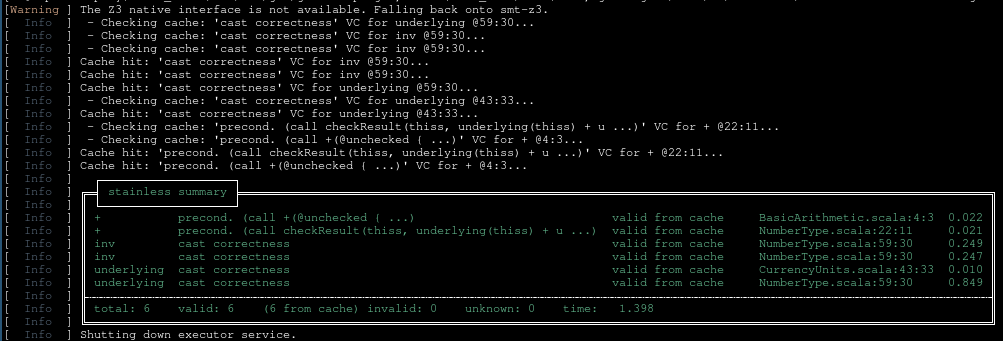
\includegraphics[width=\textwidth]{final_verify_output}
	\caption{Output of Stainless verification for addition with 0 of Bitcoin-S-Cores CurrencyUnit}
\end{figure}

The verified code.
\lstinputlisting[style=scala]{../code/currsniporig/src/main/scala/code/end/Code.scala}

But is it really the original code that we verified?
And why did we have to change that much?
This and other questions will be answered in the next chapter.


\section{Practical Challenges with Stainless}
\label{chap:appendix_arb}

In this chapter we look at the practical challenges that could occur
by using Stainless.  Since Stainless is still in development and there
is no 1.x release there might still be breaking changes and
improvements fixing problems described now.


\subsection{sbt vs JAR}

We can either use the sbt plugin or a JAR file to check code with Stainless.

Invoking the JAR on our source code Stainless will verify it.  If we
have a bigger project, this becomes really tricky, because we must
pass all files needed including the dependencies.  This is in contrast
to the sbt plugin, where we can integrate Stainless in our compilation
process.  When we call compile, Stainless verifies the code and stops
the compilation if the verification fails.

Having a static version configured in the sbt build file, every
developer has the same Stainless features available.  This should
prevent incompatibility with new or deprecated features when we use
different plugins.

So the sbt plugin has clear advantages over the JAR file since its
integrated directly.  We do not have to download it manually and find
the right version and if we bump the version we can just edit it in
the build file and every developer is on the same version again.

However, currently there are some drawbacks.  For example the sbt
plugin does not always report errors.  We will see more about that
shortly.


\subsection{Integration into Bitcoin-S}

During this work, Stainless updated the sbt plugin to support sbt
1.2.8 from 0.13.17 and Scala 2.12.8 from 2.11.12.  So this section
might be out of date now.

Stainless requires and Scala recommends Java SE Development Kit 8.
Newer Java versions won't work.

To use the latest version of the sbt tool you have to build it
locally.  You can run \texttt{sbt universal:stage} in the cloned
Stainless git repository.  This generates
\emph{frontends/scalac/target/universal/stage/bin/stainless-scalac}.

Bitcoin-S-Core uses sbt 1.2.8 and Scala 2.12.8, while Stainless sbt
plugin is on sbt 0.13.17 and Scala 2.11.12.

Sbt introduced new features in the 1.x release used by Bitcoin-S.
Most of them can be written the sbt 0.13.17 way.

The bigger problem is, due to the different Scala and sbt versions,
the following error after trying to go in a sbt shell:
\begin{verbatim}
  [warn] There may be incompatibilities among your library dependencies; run 'evicted'
         to see detailed eviction warnings.
  [error] java.lang.NoClassDefFoundError: sbt/SourcePosition
  ...
  Project loading failed: (r)etry, (q)uit, (l)ast, or (i)gnore?
\end{verbatim}

Downgrading Bitcoin-S sbt version to 0.13.17 fixes the error but then
it can not load some libraries only compiled for newer versions.  So
this would take too much time to fix and changes the Bitcoin-S code
inadvertently.

The next approach is to use the stainless cli instead of sbt.  Running
stainless on all source files does not work, because dependencies are
missing.  The parameter \emph{-classpath} can resolve it but the value
of this parameter must be the paths to all the dependencies separated
by a ':'.  Finally, \emph{core} depends on \emph{secp256k1jni},
another package of Bitcoin-S written in Java.  So this needs to be in
the source files to.

The final command looks like this in \emph{core} folder of Bitcoin-S:
\begin{lstlisting}[language=bash]
  $ stainless
    -classpath ".:$(find ~/.ivy2/ -type f -name *.jar | tr '\n' ':')"
    $(find . -type f -name *.scala | tr '\n' ' ')
    $(find ../secp256k1jni -type f -name *.java | tr '\n' ' ')
\end{lstlisting}

\emph{.ivy2} is the dependency cache of sbt.  The \emph{tr} replaces
the first char with the second so a newline with either ':' or ' '.

With this command, Stainless throws the next error:
\begin{verbatim}
  [Internal] Error: object scala.reflect.macros.internal.macroImpl in compiler mirror
             not found.. Trace:
  [Internal] - scala.reflect.internal.MissingRequirementError$.signal
             (MissingRequirementError.scala:17)
  ...
  [Internal] object scala.reflect.macros.internal.macroImpl in compiler mirror not found.
  [Internal] Please inform the authors of Inox about this message
\end{verbatim}

So we can not know how many errors will face us.  Let's go another
way, because the errors may take too much time and it might lead to a
next error.  We extract the code needed to verify a transaction mainly
the class Transaction and ScriptInterpreter with many other classes
they're depending on.

After this extraction Stainless was successfully integrated with both
sbt and JAR.

Running \texttt{sbt compile} in the project with Stainless ended
without error.  But it also ended with no output.  So we are not able
to change the code so Stainless would accept it since we do not know
what to change.

So the sbt plugin does not always complain where the JAR file did.
The open
\href{https://github.com/epfl-lara/stainless/issues/484}{issue 484 on
  GitHub} might describe exactly this error.

Now we can finally run Stainless on our code.  But this leads us to
the next findings.  We must rewrite most of the code, as described in
the previous chapters.



\section{Conclusion}
\label{chap:conclusion}

Because of the limitations of the verication tool, we could only
verify a rewritten version of the original Bitcoin-S code.  So we can
not guarantee the correctness of the addition of Satoshis with zero in
Bitcoin-S.  Not all changes we made were as trivial as the replacement
of objects with case objects.  For these non-trivial changes, as seen
for example the bound check in section \ref{sec:bound_check}, we
cannot say whether they are equivalent to the original implementation
or not.

So code should be written specically with formal verication in mind,
in order to successfully verify it.  Otherwise, it needs a lot of
changes in the software because verification is mathematical and the
current software is written mostly in object-oriented style.  Software
written in the functional paradigm would be much easier to reason
about.

Thus, either Stainless must find ways to translate more of built-in
object-oriented patterns of Scala to their verification tool or
developers must invest more in functional programming.

Also, we found that trying to verify code reveals bugs as shown in
section \ref{sec:bugfix}.  Finally, our work led to some feedback to
the Stainless developers to improve the tool.






% \begin{table}
% \caption{Table captions should be placed above the
% tables.}\label{tab1}
% \begin{tabular}{|l|l|l|}
% \hline
% Heading level &  Example & Font size and style\\
% \hline
% Title (centered) &  {\Large\bfseries Lecture Notes} & 14 point, bold\\
% 1st-level heading &  {\large\bfseries 1 Introduction} & 12 point, bold\\
% 2nd-level heading & {\bfseries 2.1 Printing Area} & 10 point, bold\\
% 3rd-level heading & {\bfseries Run-in Heading in Bold.} Text follows & 10 point, bold\\
% 4th-level heading & {\itshape Lowest Level Heading.} Text follows & 10 point, italic\\
% \hline
% \end{tabular}
% \end{table}


% \noindent Displayed equations are centered and set on a separate
% line.
% \begin{equation}
% x + y = z
% \end{equation}
% Please try to avoid rasterized images for line-art diagrams and
% schemas. Whenever possible, use vector graphics instead (see
% Fig.~\ref{fig1}).

% \begin{figure}
% 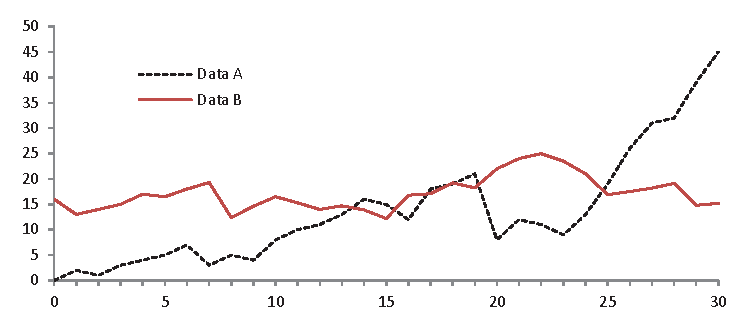
\includegraphics[width=\textwidth]{fig1.eps}
% \caption{A figure caption is always placed below the illustration.
% Please note that short captions are centered, while long ones are
% justified by the macro package automatically.} \label{fig1}
% \end{figure}

% \begin{theorem}
% This is a sample theorem. The run-in heading is set in bold, while
% the following text appears in italics. Definitions, lemmas,
% propositions, and corollaries are styled the same way.
% \end{theorem}
% %
% % the environments 'definition', 'lemma', 'proposition', 'corollary',
% % 'remark', and 'example' are defined in the LLNCS documentclass as well.
% %
% \begin{proof}
% Proofs, examples, and remarks have the initial word in italics,
% while the following text appears in normal font.
% \end{proof}
% For citations of references, we prefer the use of square brackets
% and consecutive numbers. Citations using labels or the author/year
% convention are also acceptable. The following bibliography provides
% a sample reference list with entries for journal
% articles~\cite{ref_article1}, an LNCS chapter~\cite{ref_lncs1}, a
% book~\cite{ref_book1}, proceedings without editors~\cite{ref_proc1},
% and a homepage~\cite{ref_url1}. Multiple citations are grouped
% \cite{ref_article1,ref_lncs1,ref_book1},
% \cite{ref_article1,ref_book1,ref_proc1,ref_url1}.
%

\bibliographystyle{splncs04}
\bibliography{bibliography}

\end{document}
